\documentclass[conference,compsoc]{IEEEtran}

\ifCLASSOPTIONcompsoc
  \usepackage[nocompress]{cite}
\else
  \usepackage{cite}
\fi


\ifCLASSINFOpdf
  \usepackage[pdftex]{graphicx}
  % declare the path(s) where your graphic files are
  \graphicspath{{./gra/}}
  % and their extensions so you won't have to specify these with
  % every instance of \includegraphics
  % \DeclareGraphicsExtensions{.pdf,.jpeg,.png}
\else

\fi

\usepackage{amsmath}
% \usepackage{algorithm}
% \usepackage{algorithmic}
\usepackage[ruled]{algorithm2e}
\usepackage{array}

% \renewcommand{\algorithmicrequire}{\textbf{Input:}} % Use Input in the format of Algorithm
% \renewcommand{\algorithmicensure}{\textbf{Output:}} % Use Output in the format of Algorithm

\hyphenation{op-tical net-works semi-conduc-tor}


\begin{document}

\title{Q-Learning and DDQN for Flappy Bird}


\author{\IEEEauthorblockN{HE Tianlang\IEEEauthorrefmark{1},
XU Haoran\IEEEauthorrefmark{2},
Pei Yulin\IEEEauthorrefmark{3}and 
Dong Ziwei\IEEEauthorrefmark{4}}
\IEEEauthorblockA{\IEEEauthorrefmark{1}Email: siriushe2019@gmail.com}
\IEEEauthorblockA{\IEEEauthorrefmark{2}Email: hxubh@connect.ust.hk}
\IEEEauthorblockA{\IEEEauthorrefmark{3}Email: ypeiae@connect.ust.hk}
\IEEEauthorblockA{\IEEEauthorrefmark{4}Email: zdongaj@connect.ust.hk}}

\maketitle

% As a general rule, do not put math, special symbols or citations
% in the abstract
\begin{abstract}
Reinforcement learning is trying to learn from the interaction with the environment, which is very similar to the process of human learning knowledge. Deep reinforcement learning is a combination of reinforcement learning and deep learning. In this project, we try to use reinforcement learning method and deep reinforcement learning method to train an agent to play the game Flappy Bird. We use Q-learning and Double Deep Q-Networks to train two agents separately. The agent gets the information about the location of the bird and the pipes. According to the information, agents evaluate the Q-functions. Both agents show excellent performance.
Furthermore, we discuss the performance of the two agents.
\end{abstract}


\IEEEpeerreviewmaketitle



\section{Introduction}
Reinforcement learning is a branch of machine learning. Compared with classical supervised learning and unsupervised learning problems, the biggest characteristic of reinforcement learning is learning from interaction.  Agent constantly learns knowledge according to the reward or punishment obtained in the interaction with the environment. The pattern of reinforcement learning is similar to the way of human learning knowledge. Therefore, reinforcement learning is an important way to implement artificial intelligence.
\indent 
In Reinforcement learning, if the number of the states is large, it really difficult to represent the Q-function and the agent can not determine the actions for the states never visit. deep reinforcement learning can help to solve the problem.
\indent 
The goal of the project is to learn a policy to get an agent do an excellent job on playing the game Flappy Bird. Flappy Bird is a very simple game but hard to play. The player needs to keep the bird alive. The bird automatically falls towards the ground. Every time the player clicks the bird, the bird will have the power to fly higher for a while. The bird will keep flying towards and there are pipes in front of the bird. The bird needs to fly through the area between the two pipes. If the bird hit the pipe or the ground, the bird will die. Therefore the player needs the control the bird to fly through the obstacles. Once the bird flies through a pair of pipes, the player will get one score.

\
We use the Flappy Bird game from the pygame package and reference the clone of Flappy Bird game of sourabhv in Github. The location information about the bird and pipes are given to the agent. It is very difficult to program code in the way of logical judgement to solve the problem because even the programmer itself cannot find when to click the bird to fly higher.


\begin{figure}[!t]
\centering
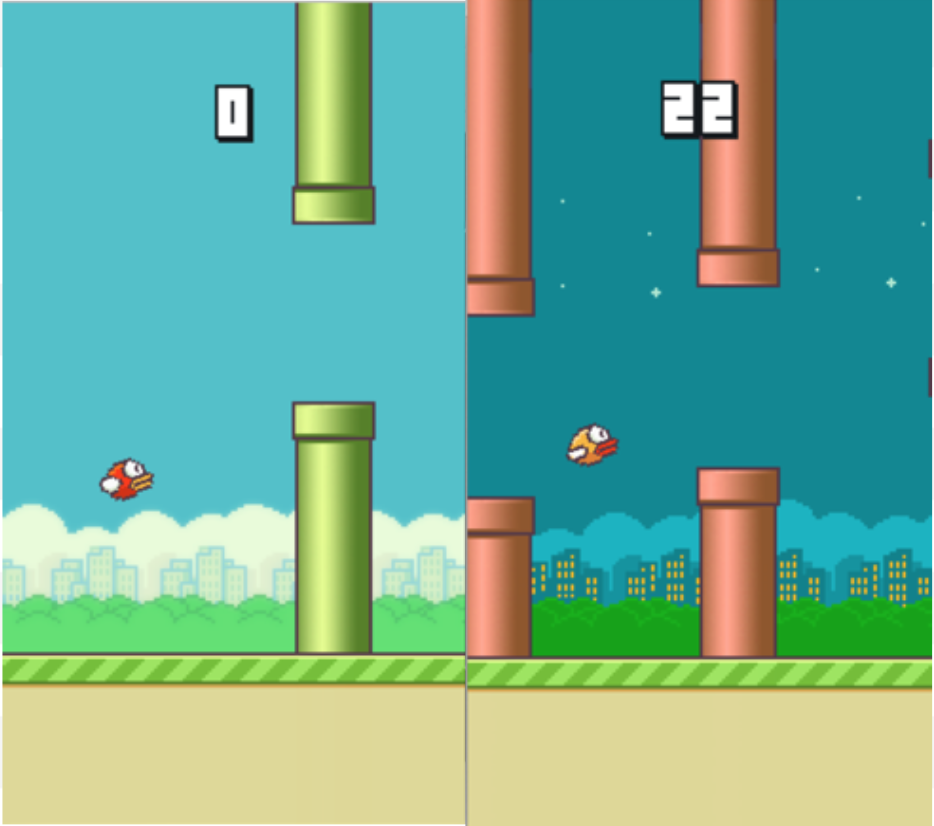
\includegraphics[width=2.5in]{fg1}
\caption{Two screenshots of the game Flappy bird.}
\label{fig_sim}
\end{figure}




\section{Related Work}
Q-learning algorithm, originally proposed by Watkins in his doctoral dissertation [1], is a very effective learning algorithm in reinforcement learning. Every step, the agent will get the reward or the punishment. The algorithm tries to find the policy the maximize the reward and avoid the punishment according to the historical experience. It’s traditional but work very well to the problems which have no single correct way to solve.
\\
\indent 
There are many people try to combine deep learning and reinforcement learning, but the first one to do it is DeepMind [2]. They try to use CNN to extract features from high-dimensional sensory inputs and then uses a reinforcement learning algorithm to learn control strategies. The trained agents have been tested in 7 Atari 2600 games and performed very well in 6 games. Agents played better than human experts in 3 games. The learning model is the combination of the CNN and Q-learning, so it’s called deep Q-network(DQN).
\\
\indent 
In 2016, DeepMind came up with the Double DQN to improve the original deep Q-network ’s performance [3]. Double DQN reduces the overestimation of the DQN and performs better.

\section{Markov Decision Process Formulation}
In Markov Decision Process [4], actions are indeterminate, and the cost function depends on the starting and ending states of the action. A MDP consists of states, actions, reward function, goal condition and a discount factor. In this section, we describe how the model is parameterized. Because we use two different methods to solve the problem, we model the game differently.

\subsection{In Q-Learning}
The state of the Flappy Bird game is represented by the bird’s coordination and pipes’ coordination. The original states we get from pygame are in JSON format and the content is shown in Table 1.


\begin{table}[!t]
% increase table row spacing, adjust to taste
\renewcommand{\arraystretch}{1.3}
\caption{The Content of the States}
\label{table_1}
\centering
% Some packages, such as MDW tools, offer better commands for making tables
% than the plain LaTeX2e tabular which is used here.
\begin{tabular}{|c|c|}
\hline
Element & Description\\
\hline
isDead & False\\
\hline
upperPipes & {'x': 488, 'y': -219}, {'x': 632.0, 'y': -154}\\
\hline
upperPipes & {'x': 488, 'y': -219}, {'x': 632.0, 'y': -154}\\
\hline
lowerPipes &{'x': 488, 'y': 211}, {'x': 632.0, 'y': 276}\\
\hline
score & 0\\
\hline
playerVelY &-9\\
\hline
playerRot & 45\\
\hline
pipeVelX & -4\\
\hline
playerAccY & 1\\
\hline
basex & 0\\
\hline
playerx & 57\\
\hline
playery &244\\
\hline
\end{tabular}
\end{table}


In the original state, there is much useless information. Before training, we preprocess the states into the ideal format. After we analyze the game, we find that we only need the distances between the bird and the next lower pipe in x-direction and y-direction to train the agent. Therefore, we transform the original state into ${gridX\_gridY\_v}$ format. ${gridX}$ represents the distance between the bird and the next first lower pipe in the x-direction. The ${gridY}$ represents the distance between the bird and the next first lower pipe in the y-direction. ${v}$ represents the velocity of the bird falling down. We define the initial state is 420\_240\_0.

\begin{figure}[!t]
\centering
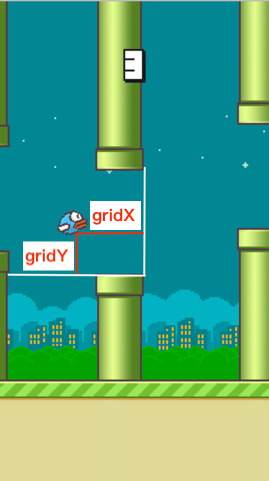
\includegraphics[width=1.5in]{fg2.png}
\caption{The pictorial description of the state information.}
\label{fig_2}
\end{figure}

\indent 
There are only two kinds of actions we can choose: click the bird to make it fly higher or do nothing. According to the game, every time the bird passes a pair of pipes, the score will be increased by 1. If the bird died, the game will be over. We should give a large punishment for letting the bird died. Therefore, we define that in the current state, if the bird is still alive, the agent can get 1 unit as a reward, otherwise, the agent gets -1000 unit as punishment. If the bird died because of crashing at the upper pipe and there is a click action in the last 3 states, the agent gets -1000 unit as punishment once. When the number of running times reaches the condition we set, the training is over. To simplify the process, we define the discount is 1.

\begin{table}[!t]
% increase table row spacing, adjust to taste
\renewcommand{\arraystretch}{1.3}
\caption{Model Definition for Q-Learing}
\label{table_2}
\centering
% Some packages, such as MDW tools, offer better commands for making tables
% than the plain LaTeX2e tabular which is used here.
\begin{tabular}{|c|p{130pt}|}
\hline
Element & Description\\
\hline
state(s) & gridX\_gridY\_v
\\
\hline
Initial state(${s_0}$) &420\_240\_0
\\
\hline
Action(a) & Click or do nothing\\
\hline
Reward function(r) & Alive: 1;Died: -1000\\
 & Alive but take action click leading died: -1000\\
\hline
Goal condition & the number of running times\\
(End(s)) &reaches the condition\\
\hline
Discount factor(${\gamma}$) &1 \\
\hline
\end{tabular}
\end{table}

\subsection{In Double Deep Q-Network}
In DDQN we also need to preprocess the original states and we decide to use [gridX, gridY, v, playerRot] to represent the states. Compared with the states in Q-learning, the rotation of the bird is contained in the states. The starting state is automatically calculated for the bird and the random initial pipes. The actions are the same as the actions in Q-learning. 
\\
\indent 
In our analysis, if the bird already gets high scores, the agent should get a higher reward for maintaining the scores. So we define the reward is the scores the bird maintained in the current states. In case the bird is flying too high, every time the gridY is larger than 250, the reward will minus 200. If the bird died, the agent will get -1000 for punishment.
\\
\indent 
When the number of running times reaches the condition we set, the training is over. For the performance of the training, the discount factor is 0.99.

\begin{table}[!t]
% increase table row spacing, adjust to taste
\renewcommand{\arraystretch}{1.3}
\caption{Model Definition for Q-Learing}
\label{table_3}
\centering
% Some packages, such as MDW tools, offer better commands for making tables
% than the plain LaTeX2e tabular which is used here.
\begin{tabular}{|c|p{150pt}|}
\hline
Element & Description\\
\hline
state(s) & [gridX, gridY, v, playerRot]
\\
\hline
Initial state(${s_0}$)&Random 
\\
\hline
Action(a) & Click or do nothing\\
\hline
Reward function & Alive and ${gridY <= 250}$: reward = score ;\\
 (r) & Alive and ${gridY > 250}$: reward = score - 200;\\
  & Died: reward = score -1000;\\
\hline
Goal condition & the number of running times\\
(End(s))&  reaches the condition\\
\hline
Discount factor(${\gamma}$) & 0.99 \\
\hline
\end{tabular}
\end{table}

\section{Method}

\subsection{Q-Learning}

In Q-learning algorithm, Q-function ${Q(s, a)}$ represents the utility of doing action ${a}$ in state ${s}$. We need to maintain every action’s Q-function in every state s. The representation is a kind of table. We always want to maximize the utility. When we need to choose an action at a specific state, we can look up the table to find the best action that gives us the highest utility. According to the Q-learning algorithm, we will update the Q-function as equation (1).

\begin{equation}
Q(s,a)=(1-\mu)*Q(s,a) + \mu(r+ \gamma * \mathop{max}_{a'}Q(s',a'))
\end{equation}

In equation (1), ${\mu}$ represent the learning rate. Learning rate control the balance between the new knowledge and the old experience.${Q(s',a')}$ represents the Q-function of next state ${s'}$ after taking action ${a'}$. Before we stop the training, the Q-function keeps on updating. The algorithm 1 shows the whole procedure for training the agent.

\begin{algorithm}
\caption{Q-Learning for Flappy Bird}
\label{alg:A1}
Initialize ${Q(s,a)}$\\
\For{the number of running times smaller than the condition}{
	for state ${s}$, pick action ${a}$ which has maximal ${Q(s,a)}$\\
	put [${s}$,${a}$,${s'}$] into the actions list\\
	bird gets a new state ${s'}$\\
  \If{the bird is dead}{
      \ForEach{state record [${s}$,${a}$,${s'}$] in the actions list} {
		    ${NewQvalue = r+ \gamma * \mathop{max}_{a'}Q(s',a')}$\\
		    ${Q(s,a)=(1-\mu)*Q(s,a) + \mu * NewQvalue}$
      }
      set actions list to empty
	}
}
\end{algorithm}

\subsection{Double Deep Q-Network}
Q-learning algorithm gives a good way to train the agent, but we need to store all the Q(s, a) for every possible state. The agent can only choose a random action for the states never visited. So, we try to use Double Deep Q-Network to train the agent.
\subsubsection{Deep Q-Network with target network}
 
 \

\indent 
DDQN is the improve version of Deep Q-Network(DQN). DQN is a value based algorithm. DQN algorithm tries to use a neural network to find an optimal estimation ${Q(s, a; \theta)}$ of Q-function for every state. For training the neural network we need to find an objective function, so that ${Q(s, a; \theta)}$ can get closer to the true target ${Q(s, a)}$. Because we don’t know the target, so the algorithm use TD target in equation (2).
\begin{equation}
y=r(s,a) + \gamma * \mathop{max}_{a'}Q(s',a';\theta)
\end{equation}

According to equation (2), we can get the loss function equation (3).

\begin{equation}
\begin{align}
L(\theta)&=(y-Q(s,a;\theta))^2\\
&=(r(s,a) + \gamma * \mathop{max}_{a'}Q(s',a';\theta)-Q(s,a;\theta))^2
\end{align}
\end{equation}
The upating rule is equation (4).

\begin{equation}
\theta  \leftarrow \theta - \alpha\nabla_{\theta}{L(\theta)}
\end{equation}

Because the target is always changing, the algorithm defines a target network that has the same structure as DQN. let ${\theta^-}$ be the parameters. We need to set ${\theta^- = \theta}$ once in a while.So the TD target is now defined as equation (5).
\begin{equation}
y=r(s,a) + \gamma * \mathop{max}_{a'}Q(s',a';\theta^-)
\end{equation}

\subsubsection{Experience Replay}
 
 \

\indent There is a problem with the training process. In reinforcement learning, the experiences we got from the same episode is step by step. They are very correlated. This kind of data will lead to inefficient training. So the idea of experience replay is used to update the parameters. Every time we get a new state, we put the state into a fixed size buffer. If the buffer is full, we randomly get experiences from the buffer to train the neural network. As a result, our experiences are no longer likely to be correlated.

\subsubsection{DDQN}
  
 \

\indent In DQN, the algorithm use equation (5) to estimate the TD target which causes the problem of overestimation of the ideal value. In order to maximize the Q-function of the state s, we always want to choose the best action. In equation (5), the action a is chosen when it can maximize the Q-function of the target network. In DDQN,  the action a is chosen when it can maximize the Q-function of the training network of the DQN, which makes the TD target is much closer to the ideal value. The TD target is shown in equation (6)
\begin{equation}
\begin{align}
y &=r(s,a) + \gamma * Q(s',a^*;\theta^-)
\\
a^*&=\mathop{\arg\max}_{a'} Q(s',a';\theta)
\end{align}
\end{equation}
The algorithm 2 shows the procedure of using DDQN in the flappy bird.

\begin{algorithm}
\caption{DDQN for Flappy Bird}
\label{alg:A1}
Initialize: ReplayBuffer is empty\\
Initialize: gamma = 0.99\\
Initialize: define trainNetwork with weight ${\theta}$\\
Initialize: define targetNetwork which is the same as trainNetwork with weight ${\theta^-}$\\
\ForEach{episode ${e\in [1,2,...400]}$}{
when state changes, get bird’s old state ${s}$, action ${a}$, new state ${s'}$, ${score}$ and exploreTime.\\
${reward = score }$\\
\If{girdY ${>}$ 250}{${reward = reward -200}$}
\eIf{the bird is dead} 
	{${\theta^- = \theta}$\\put[${s}$, ${a}$, ${reward-1000}$,${s'}$,Alive or Dead] into ReplayBuffer}
	{put[${s}$, ${a}$, ${reward}$,${s'}$,Alive or Dead] into ReplayBuffer}
\If{exploreTime ${>}$ 1000}{
	get random samples from ReplayBuffer\\
	\ForEach{sample ${sam \in samples}$} {
	\eIf{the bird is dead}
	{${y[sam][a] = reward}$}
	{
		get the action ${a^*}$ that maximize the ${trainQvalue}$ of ${s'}$ in trainNetwork\\
		get the ${targetQvalue}$ in targetNetwork with ${s'}$ and ${a^*}$\\
		${y[sam][a^*] = reward + \gamma * targetQvalue}$
	}
	}
train the trainNetwork with y
}
\If{${score >=10}$ and ${score\,mod\,10 == 0}$}{
    save the model\\
  }
}
\end{algorithm}
 
\subsection{Exploration and Exploitation}
When we training, we always want to explore new states. In the same time, we want to use our experience to get better performance. So we define the probability ${\epsilon}$. In training, we select a random action with probability ${\epsilon}$ and choose the optimal action from our training model with probability ${1-\epsilon}$. 
\

\indent Besides, we find that if we choose action click, the bird will fly higher in the next several states. So we give less probability in selecting click among the random choices. 


\section{Result}
\indent A video can be found at the following link: http://youtube.com. Our metric for evaluating the performance of the two algorithm is the game scores. Both of the two agents give excellent performance.
\subsection{Result of Q-learning}
\indent In Q-learning, we define a QAgent to play the game. Table 4 shows the specific definition of QAgent.

\begin{table}[!t]
% increase table row spacing, adjust to taste
\renewcommand{\arraystretch}{1.3}
\caption{The definition of the QAgent}
\label{table_4}
\centering
% Some packages, such as MDW tools, offer better commands for making tables
% than the plain LaTeX2e tabular which is used here.
\begin{tabular}{|c|c|}
\hline
Attribute and function & Description\\
\hline
self.dumpNumber = 30& the time to save model\\
\hline
self.gameCount = 0 & the number of the game iterations\\
\hline
self.discount = 1.0 & discount factor\\
\hline
self.lState = 420\_240\_0 & last state\\
\hline
self.lAction = 0 & last action\\
\hline
self.actions = [] & actions list\\
\hline
self.istrain = istrain & whether it is a training\\
\hline
load\_qvalues(self) & load value from qvalues.json\\
\hline
dump\_qvalues(self, exit = False) & save model\\
\hline
act(self, cs) & get action from state\\
\hline
update(self, dump\_qvalues = True) & updating model\\
\hline
stateToGrid(self,x, y, x1, y1, x2, y2, v) &preprocess the states\\
\hline
\end{tabular}
\end{table}

\indent We first let the QAgent with ${\epsilon}$  play the game 3300 times. When the QAgent chooses random actions, the QAgent may die. So we set the ${\epsilon}$  is 0.008. Because of the randomness, the performance while training is not so good. Figure 3 shows the performance while training. We can see that the scores slowly increases while playing. The maximal score is 98 and the average score is 5.

\begin{figure}[!t]
\centering
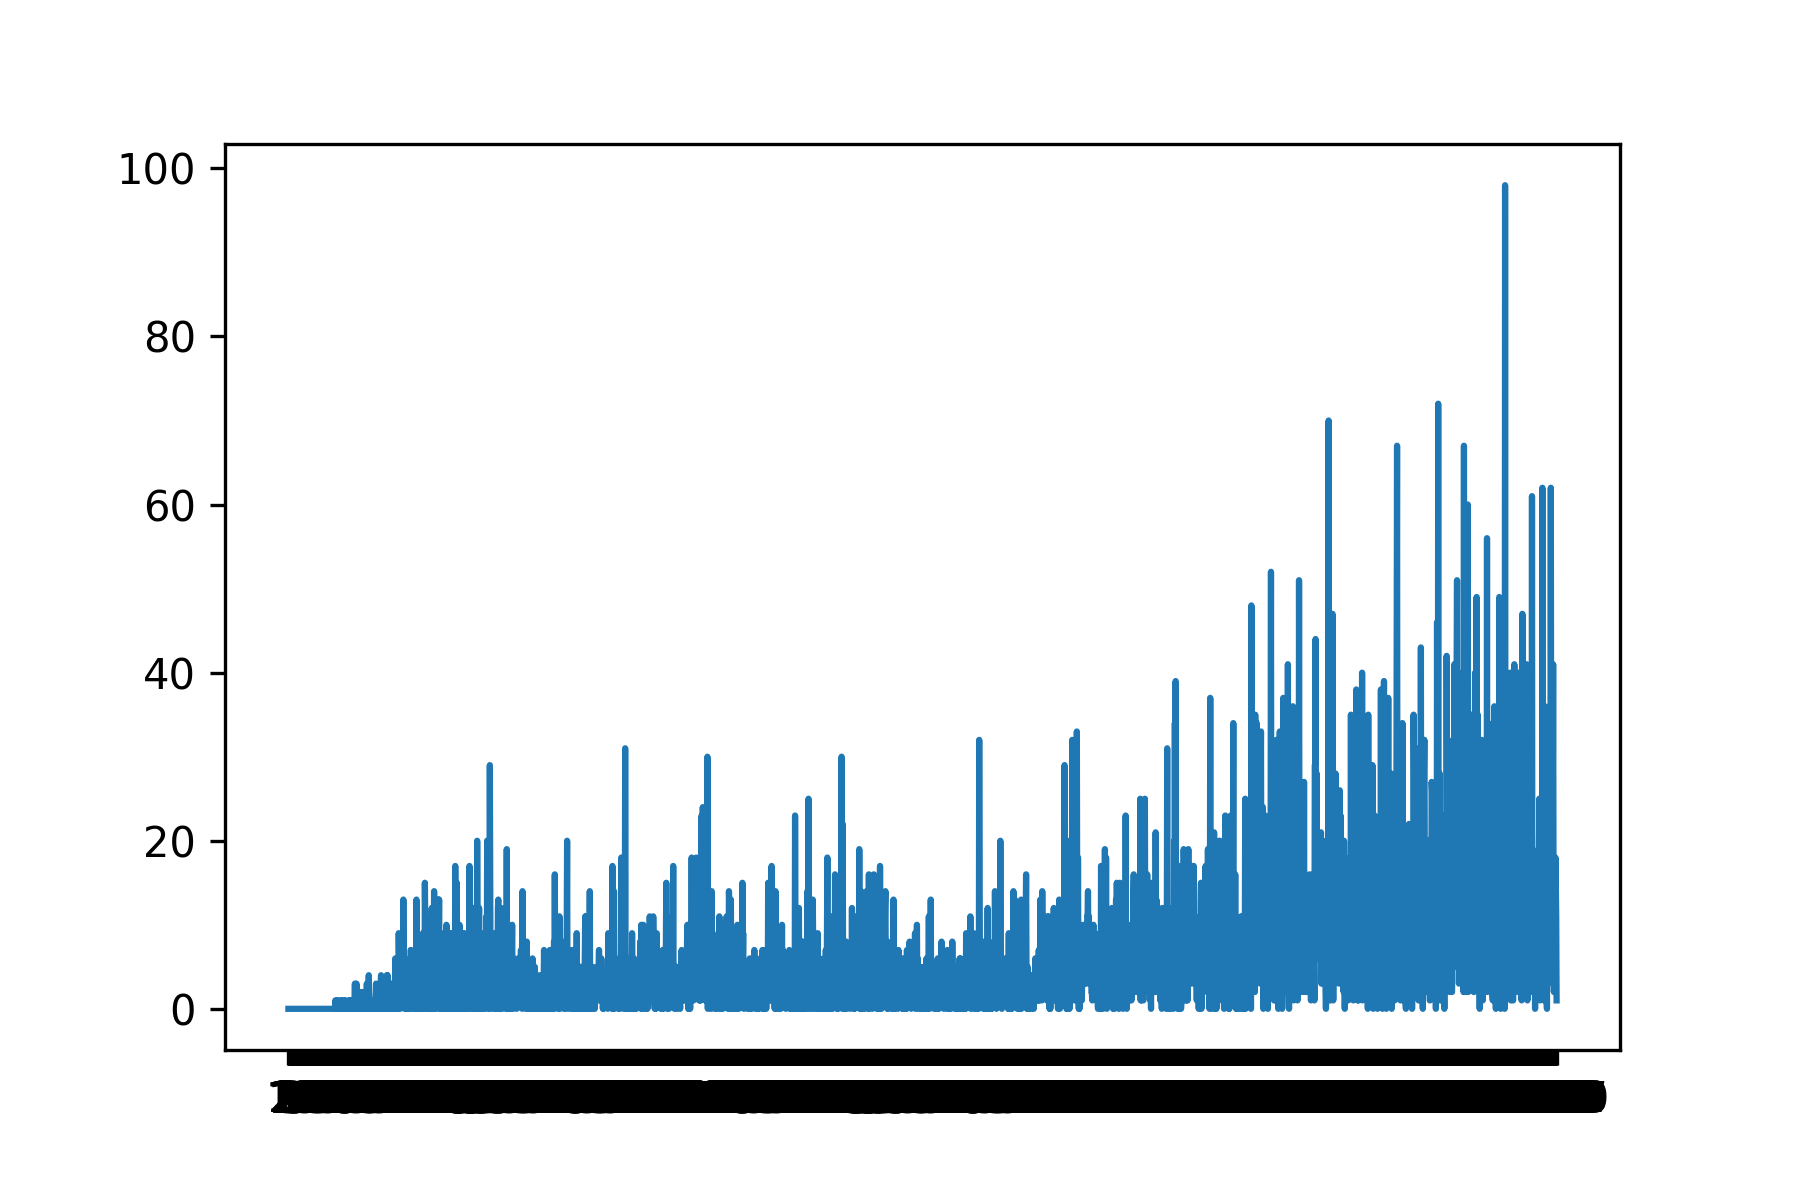
\includegraphics[width=2.5in]{Qlearn_Ep_result.png}
\caption{The scores of QAgent with ${\epsilon}$ after QAgent played 3300 times.}
\label{fig3}
\end{figure}

\indent After we train the QAgent with ${\epsilon}$ , we use QAgent which totally depend on the experience to play the game. The result is shown in Figure 4.  After 120 games, the average score is 635 which is much higher than 98. The maximal score is 4171 which shows excellent performance of QAgent.

\begin{figure}[!t]
\centering
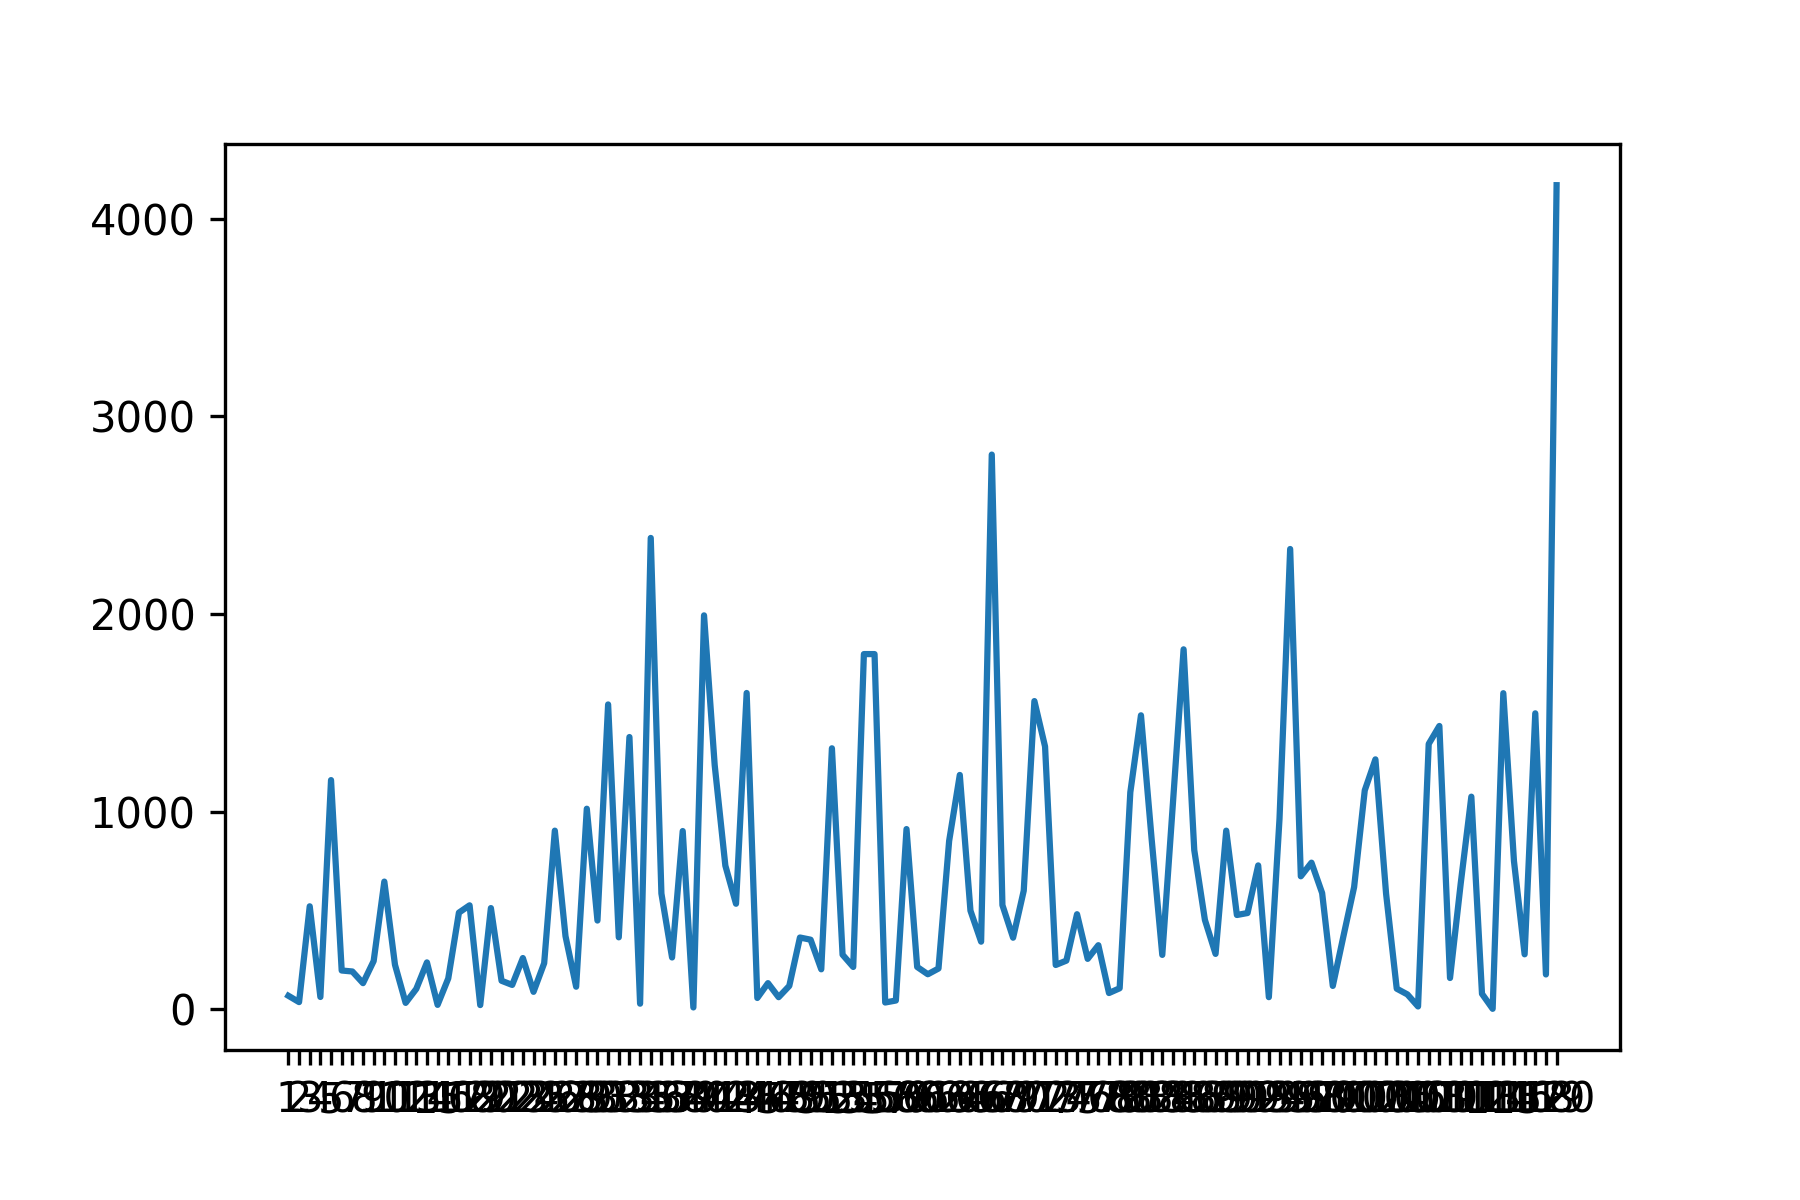
\includegraphics[width=2.5in]{Qlearn_noEp_result.png}
\caption{The scores of QAgent without ${\epsilon}$ after QAgent played 120 times.}
\label{fig3}
\end{figure}

\subsection{Result of DDQN}
In DDQN, we define a DeepAgent to play the game and a DeepTrain model to train the DeepAgent. Table 5 shows the specific definition of DeepAgent and Table 6 shows the specific definition of DeepTrain model.

\begin{table}[!t]
% increase table row spacing, adjust to taste
\renewcommand{\arraystretch}{1.3}
\caption{The definition of the DeepAgent}
\label{table_5}
\centering
% Some packages, such as MDW tools, offer better commands for making tables
% than the plain LaTeX2e tabular which is used here.
\begin{tabular}{|p{110pt}|p{110pt}|}
\hline
Attribute and function & Description\\
\hline
self.model=DeepTrain() & define the training model\\
\hline
self.syncCount=0 & the count of the states’ change\\
\hline
self.tryTime=0 & the number of the game iterations\\
\hline
self.exploreTime=0 & the times of the random actions the agent choosee\\
\hline
onStateChange(self, oldState, action, newState) & some process needs to do when state changes\\
\hline
getNextAction(self, state) & return the action\\
\hline
processState(self,rawState) & preprocess State\\
\hline
onDone(self,reward) & some process needs to do when bird died\\
\hline
\end{tabular}
\end{table}

\begin{table}[!t]
% increase table row spacing, adjust to taste
\renewcommand{\arraystretch}{1.3}
\caption{The definition of the DeepTrain model}
\label{table_5}
\centering
% Some packages, such as MDW tools, offer better commands for making tables
% than the plain LaTeX2e tabular which is used here.
\begin{tabular}{|p{110pt}|p{110pt}|}
\hline
Attribute and function & Description\\
\hline
self.stateShape=4 & the size of the state\\
\hline
self.actionSpaceNum=2 & the size of action space\\
\hline
self.gamma = 0.99 & the discount factor\\
\hline
self.epsilon = 0.2 & epsilon(${\epsilon}$)\\
\hline
self.epsilon\_decay = 0.001 & the decay amount of epsilon\\
\hline
self.epsilon\_min = 0.0001 & the minimum of epsilon\\
\hline
self.learingRate = 0.0001 & learning rate\\
\hline
self.replayBuffer = deque(maxlen=60000) & replay Buffer\\
\hline

self.trainNetwork = self.createNetwork() & the network used to train the Qvalue\\
\hline

self.numPickFromBuffer = 32*2 & the size of the samples picked from the replay Buffer\\
\hline

self.targetNetwork = self.createNetwork() & the target network\\
\hline

self.targetNetwork.set\_weights& make the parameters of the\\
(self.trainNetwork.get\_weights()) & target network same as the trainNetwork\\
\hline

createNetwork(self) & create a neural network\\
\hline

getBestAction(self, state) & return the action\\
\hline
trainFromBuffer(self) & train the model\\
\hline
\end{tabular}
\end{table}

In DDQN, we set the epsilon is 0.2 at first and the epsilon will minus 0.001 when the DeepAgent died with a score higher than 0. Eventually, the epsilon will decay to 0.001. We let the DeepAgent play the game 1292 times. Figure 5 shows the performance while training.

\begin{figure}[!t]
\centering
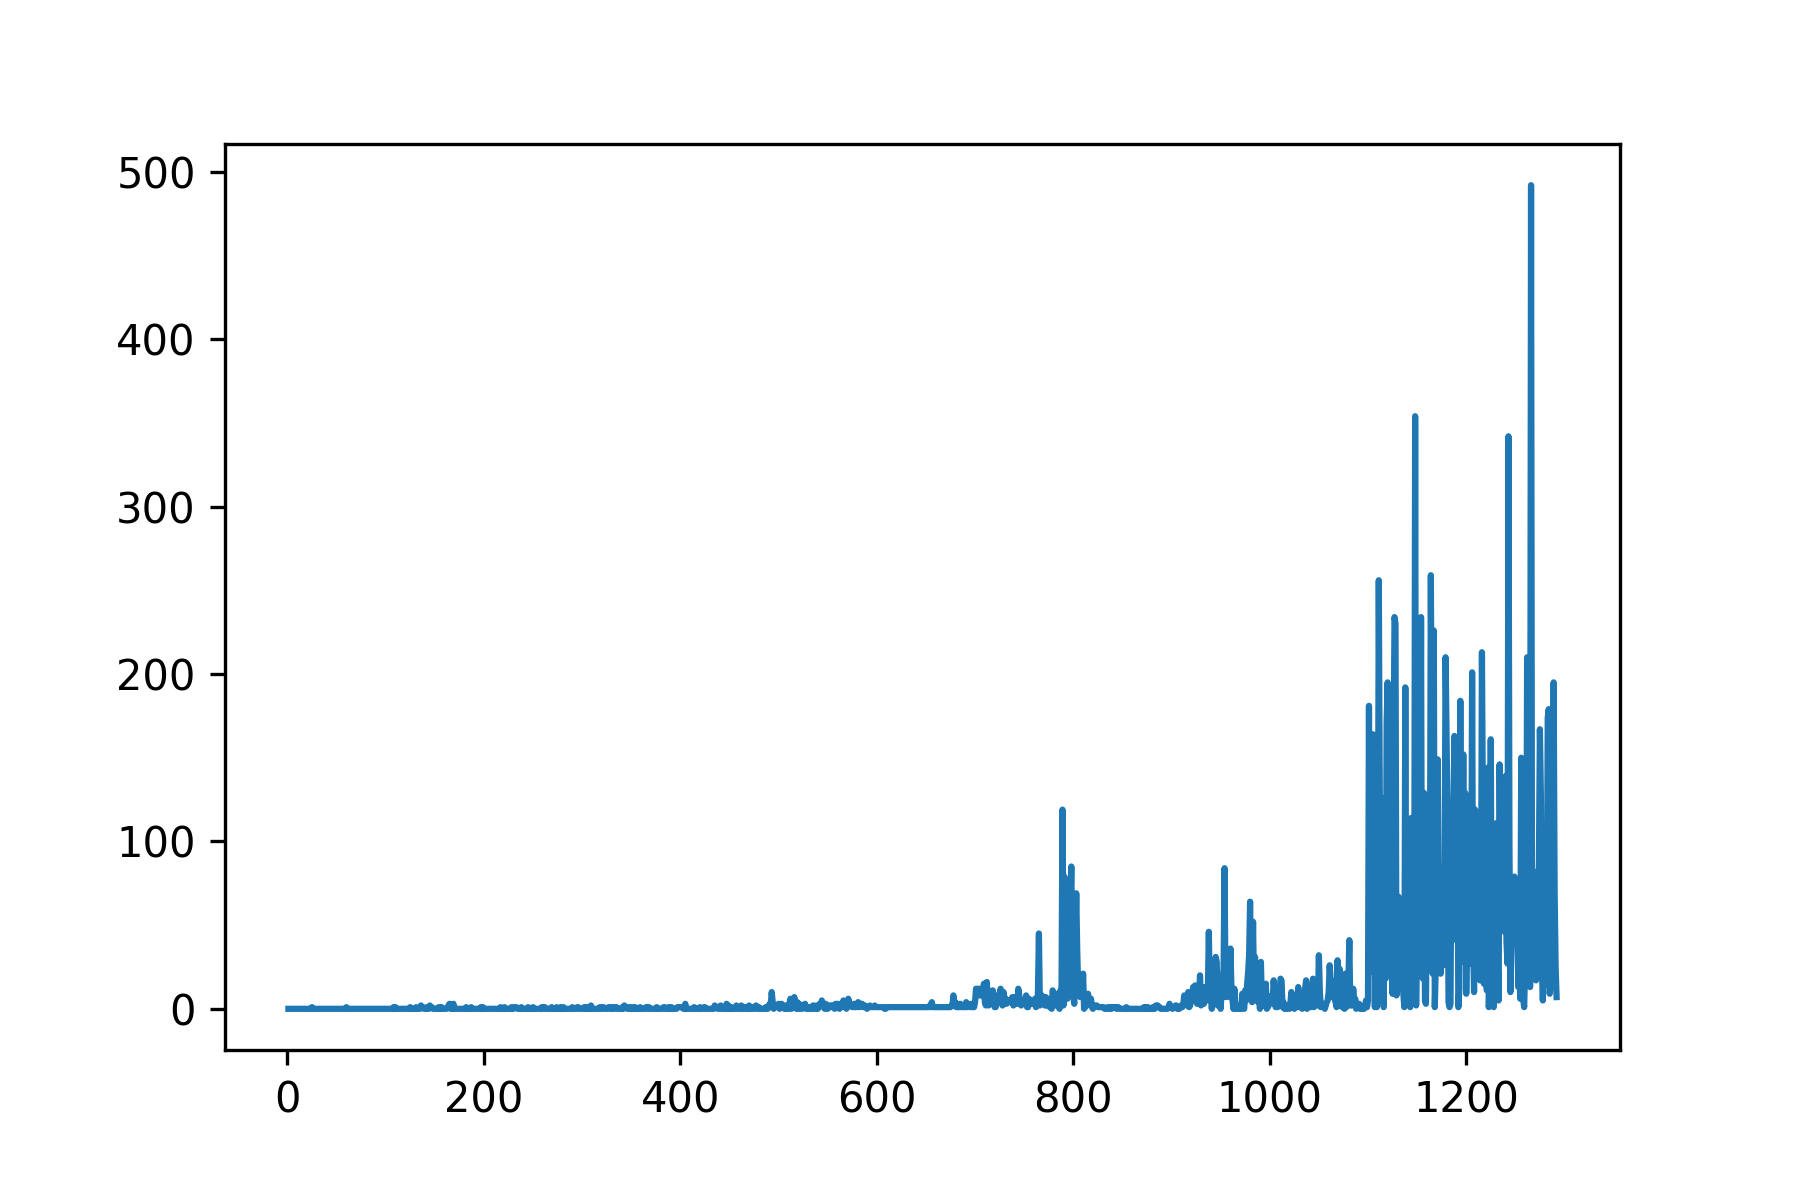
\includegraphics[width=2.5in]{DDQN_result.png}
\caption{The scores of DeepAgent after DeepAgent played 1292 times.}
\label{fig5}
\end{figure}


Due to the effectiveness of epsilon, the DeepAgent shows a really bad performance at the beginning. After playing 800 times, the DeepAgent begin to get more scores. In the last 200 iterations,  the average score is 72. In DDQN, the input feature dimension is 4 and neural network layers have at most 64 hidden units which mean we have plenty of parameters to train. So the neural network needs much more time to train.



\section{Conclusion}

We can successfully play the game Flappy Bird by using the two agent we trained. Both of them give better performance than human. Q-learning and DDQN are used to train agents. The two algorithms have different parameters and different training process.  Because the neural network needs much more time to train, we can not compare them according to the number of the game iterations. According to Figure 3 and Figure 5, we can roughly find that QAgent is improved steadily while DeepAgent gets higher scores during training. We can make a wild guess that the DeepAgent will show better performance if it get more time to train.
\begin{figure}[!t]
\centering
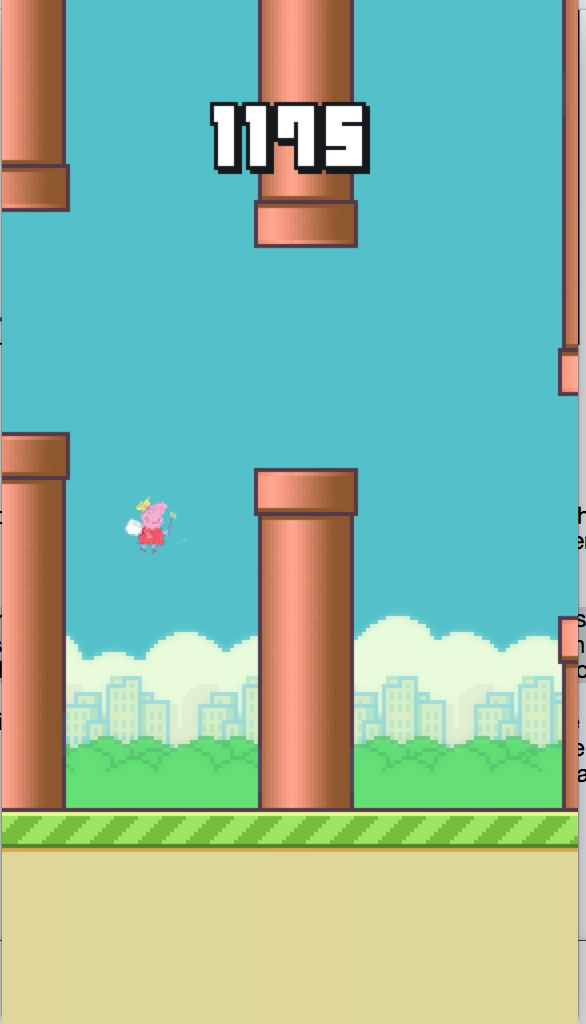
\includegraphics[width=1.5in]{f3}
\caption{The screen shot of Flappy Bird}
\label{fig_7}
\end{figure}

The preprocess with the game Flappy Bird and the training of DDQN is done by Pei Yulin. The training of Q-learning is done by HE Tianlang and XU Haoran. The method analysis and report writing are done by DONG Ziwei. The video is made by  XU Haoran.

\indent 

\indent 
% use section* for acknowledgment
\ifCLASSOPTIONcompsoc
  % The Computer Society usually uses the plural form
  \section*{Acknowledgments}
\else
  % regular IEEE prefers the singular form
  \section*{Acknowledgment}
\fi

The authors wish to thank Professor Nevin L. Zhang from the Department of  Computer Science and Engineering, The Hong Kong University of Science and Technology, for providing the necessary advice.  The authors also like to thank the sourabhv for providing the clone of the Flappy Bird game on Github. The authors also would like to thank SarvagyaVaish for providing the Q-learning analysis on game Flappy Bird.
  


\begin{thebibliography}{1}

\bibitem{IEEEhowto:kopka}
Watkins C J C H, Dayan P. Q-learning[J]. Machine learning, 1992, 8(3-4): 279-292.
\bibitem{IEEEhowto:kopka}
Mnih V, Kavukcuoglu K, Silver D, et al. Playing atari with deep reinforcement learning[J]. arXiv preprint arXiv:1312.5602, 2013.
\bibitem{IEEEhowto:kopka}
Van Hasselt H, Guez A, Silver D. Deep reinforcement learning with double q-learning[C]//Thirtieth AAAI Conference on Artificial Intelligence. 2016.
\bibitem{IEEEhowto:kopka}
Russell S J, Norvig P. Artificial intelligence: a modern approach[M]. Malaysia; Pearson Education Limited,, 2016.

\end{thebibliography}




% that's all folks
\end{document}


